\documentclass{article}
\usepackage[landscape]{geometry}
\usepackage{geometry}
\usepackage[table]{xcolor}% http://ctan.org/pkg/xcolor
\usepackage{fancyhdr}
\usepackage{amsmath, amssymb}
\usepackage{graphicx}
\usepackage{color}
\usepackage{longtable}
\definecolor{bg}{rgb}{0.89, 0.95, 0.71} % background e3f3b4
\definecolor{ac}{rgb}{0.50, 0.18, 0.41} % accent c491b6
\definecolor{rc}{rgb}{0.77, 0.57, 0.71} % rule 7f2f69
\usepackage{listings}
%catalan packages
\usepackage[catalan]{babel}
\usepackage[T1]{fontenc}
\usepackage[utf8]{inputenc}
%
\lstset{
       basicstyle=\small\ttfamily,
       xleftmargin=1em,
       }
\lstdefinestyle{latex}{language=TeX,
                       backgroundcolor=\color{bg},
                       basicstyle=\small\ttfamily,
                       frame=leftline,
                       xleftmargin=1.4em,
                       framexleftmargin=.8em}
\lstdefinestyle{cmdline}{
                         }
\usepackage{url}
\usepackage[pdftex,
            bookmarks,
            colorlinks=true,
            linkcolor=black,
            plainpages = false,
            pdfpagemode = UseNone,
            pdfstartview = FitH,
            citecolor = ac, urlcolor = ac, filecolor = ac]{hyperref}

\usepackage[para]{footmisc}
% Change horiz room between fn mark and fn hskip from .5em
% Suggested to RF making this settable
\makeatletter
\long\def\@makefntext#1{\leavevmode
\@makefnmark\nobreak
\hskip.05em\relax#1%
}
\makeatother
%\newcommand{\texdoc}[1]{\/\footnote{\protect\texttt{#1}}}
\newcommand{\citelink}[3]{\href{#1}{#2}~\cite{#3}}
\newcommand{\bibliolink}[2]{\href{#1}{\nolinkurl{#1}}, \href{#1}{#2}}

\setlength{\parskip}{0.75ex}
\makeatletter 
\makeatother
\setcounter{secnumdepth}{0}

\newlength{\rulelength}
\setlength{\rulelength}{\linewidth}
\addtolength{\rulelength}{9.5em}
\title{Must Know}
\author{INS Vilafant 18/19}
\date{\today}

\pagestyle{plain}
\begin{document}
\thispagestyle{empty}
%\maketitle
\setlength{\unitlength}{1in}

\makeatletter
\vspace*{3ex}
\par\noindent{\hspace*{-1.5em}\LARGE\bf \@title}
\vspace*{-1.2ex}
\par\noindent{{\hspace*{-1.5em}\rule{\rulelength}{1.05pt}}}
\vspace*{-.5ex}
\par\noindent{\hspace*{-1.5em}\large \@author}
\vspace*{5ex}
\makeatother







\begin{center}
	\begin{longtable}{ | l |l|l|}
		\hline
		\cellcolor{gray}\textbf{Topic} & \cellcolor{gray}\textbf{Resum / Equació} &  \cellcolor{gray}\textbf{Gràfics} \\
		\hline
    \href{http://proyectodescartes.org/EDAD/materiales_didacticos/EDAD_3eso_cat_progressions-JS-LOMCE/index.htm}{Successions} & Aritmètica: $a_n=a_1 \cdot (n-1) \cdot d$ & \\
        & Geomètrica: $a_n=a_1 \cdot r^{n-1}$ & \\
        \hline
     Àrees de figures planes & & \\
     & $A_{quadrat}=c^2$ & \\
     & $A_{rectangle}=b\cdot h$ & \\
     & $A_{triangle}=\frac{b\cdot h}{2}$ & \\
     & $A_{rombe}=\frac{D\cdot d}{2}$ & \\
     & $A_{trapezi}=\frac{(B+b)\cdot h}{2}$ & \\
     & $A_{cercle}=\pi \cdot r^2$ & \\
     \hline
     Àrees i Volums de cossos geomètrics & & \\
     & $A_{cub}=6\cdot c^2 \qquad V_{cub}=c^3$ & \\
     & $A_{prisma}=2\cdot A_{base}+n\cdot A_{rec. lat.} \qquad V_{prisma}=a\cdot b \cdot c$ & \\
     & $A_{piramide}=A_{base}+n\cdot A_{triang. lat.} \qquad V_{piramide}=\frac{1}{3} A_{base} \cdot h$ & \\
     & $A_{cilindre}=2 \cdot \pi r^2+2\cdot \pi \cdot r \cdot h \qquad V_{cilindre}=\pi \cdot r^2 \cdot h$ & \\
     & $A_{con}=\cdot \pi r^2+ \pi \cdot r \cdot g \qquad V_{con}=\frac{1}{3}\pi \cdot r^2 \cdot h$ & \\
     & $A_{esfera}=4 \cdot \pi r^2 \qquad V_{esfera}=\frac{4}{3}\pi \cdot r^3$ & \\
     
     \hline   

    Identitats notables     &$(a+b)^2=a^2+b^2+2ab$ & \\
    & $(a-b)^2=a^2+b^2-2ab$ & \\
    & $(a+b)\cdot (a-b)=a^2-b^2$ & \\
        \hline
        Equació de segon grau     &$ax^2+bx+c=0$ & \\
        & $x=\frac{-b \pm \sqrt{b^2-4ac}}{2a}$ & \\
        
            \hline

    \href{http://proyectodescartes.org/EDAD/materiales_didacticos/EDAD_4eso_cat_polinomios-JS-LOMCE/index.htm}{Descomposició factorial de polinomis}& 1. Treure factor comú & \\
    & 2. Identificar identitats notables & \\
    & 3. Descomposició per Ruffini $(x-a)$ & \\
    \hline
    Trigonometria & Relacions trigonomèriques importants& \\
    & $\sin^2 x + \cos^2 x=1  $& 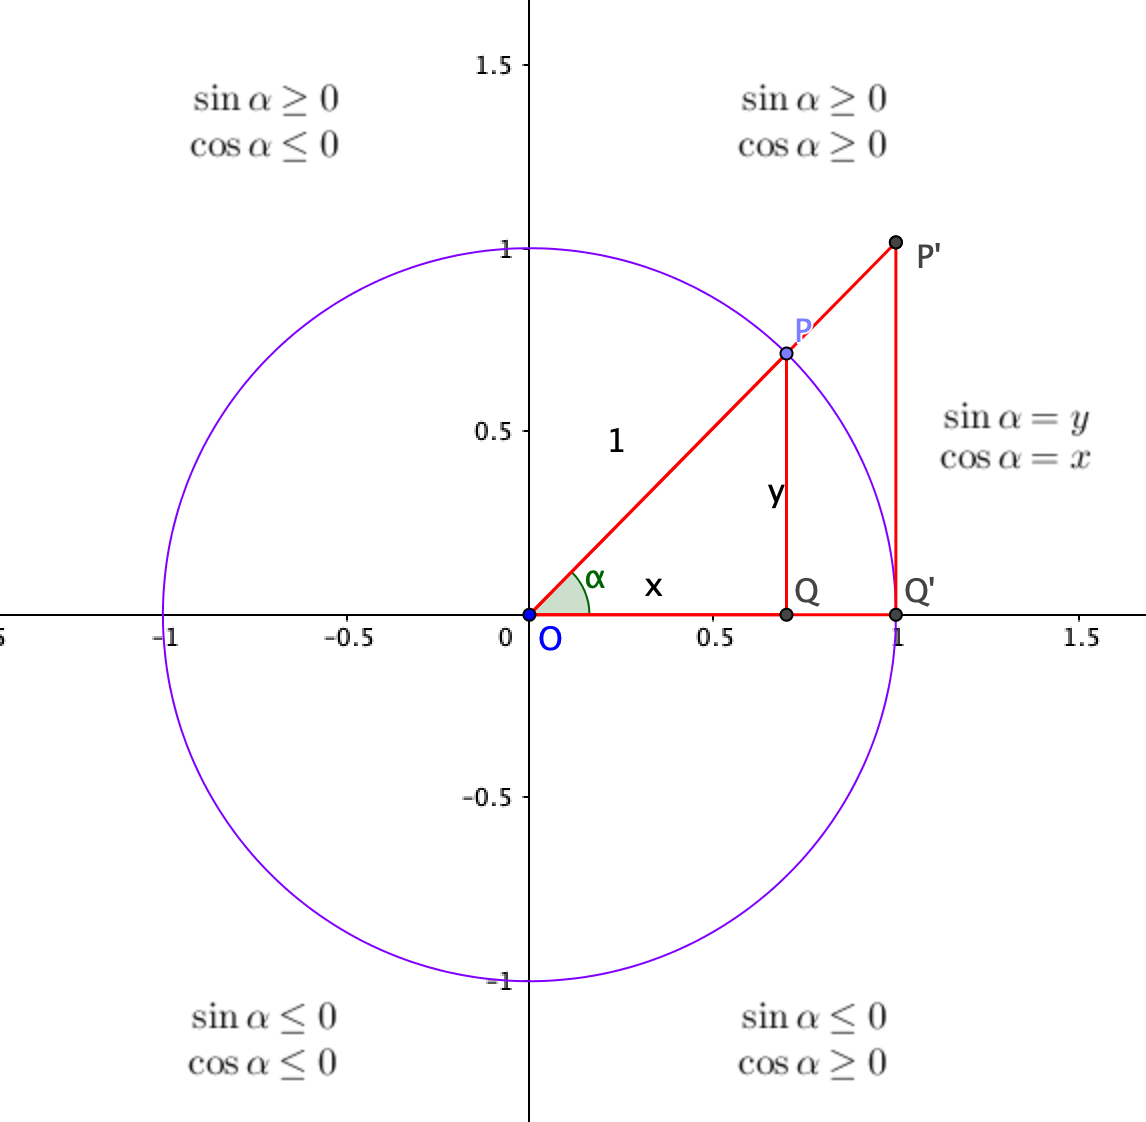
\includegraphics[width=0.2\textwidth, height=30mm]{circumf_unitat.png}\\
    & $\cos(2x) =\cos^2 x-\sin^2 x$& \\
    & $\sin(2x)=2\cos x \sin x$& \\
    \hline
    Representació gràfica de funcions & & \\
    & Domini: $\begin{cases} \frac{f(x)}{g(x)}\rightarrow D=\mathbb{R}-zeros\qquad g(x)\\ \sqrt{f(x)}\rightarrow D=x | f(x) \ge 0\\ log(f(x)) \rightarrow D=x | f(x) > 0 \end{cases}$ & \\
    & Punts de tall amb els eixos: eix $x\rightarrow f(x)=0$, eix $y\rightarrow f(0)$& \\
    & Simetria parell $f(x)=f(-x)$, simetria senar $f(x)=-f(-x)$& \\
    & Ass. verticals $\rightarrow \lim_{x\to a }f(x)=\pm \infty$& \\
    & Ass. horitzontals $\rightarrow \lim_{x\to \pm \infty }f(x)=a$& \\
    & Creixement i decreixement $\rightarrow$ signe $f^{,}(x)$&\\
    & Màxims i mínims $\rightarrow$ $f^{,}(x)=0$ i $f^{,,}(x)<0$ o $f^{,,}(x)>0$&\\
    & Punts d'inflexió $\rightarrow$ $f^{,,}(x)=0$ i $f^{,,,}(x)\neq 0$&\\
    & Concavitat i convexitat $\rightarrow$ signe $f^{,,}(x)$&\\
        \hline
    Translacions en els eixos& & \\
    & $f(x+a), a>0\rightarrow$ Trasllada $f(x)$ $a$ unitats cap a l'esquerra, eix $x$& \\
    & $f(x)+a, a>0\rightarrow$ Trasllada $f(x)$ $a$ unitats cap a dalt, eix $y$& \\
    \hline
    Rectes& & \\
    &$y=mx+n$&\\
    &$Ax+By-C=0\rightarrow \overrightarrow{v}=(-B,A)\qquad m=-\frac{A}{B}$&\\
    \hline
    Paràboles& & 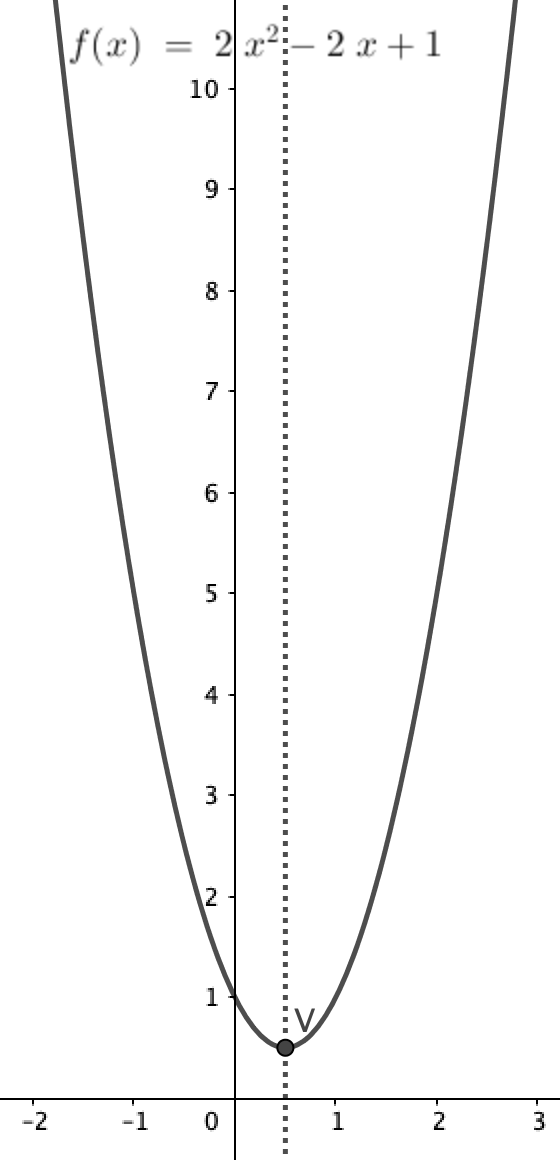
\includegraphics[width=0.2\textwidth, height=30mm]{eq_2n_grau.png}\\
    &$y=ax^2+bx+c$&\\
    &vèrtex$\rightarrow x=-\frac{b}{2a}$&\\
    &Tall eix x: $ax^2+bx+c=0$; Tall eix y: $(0,c)$&\\
    &$a>0\rightarrow \cup \qquad a<0\rightarrow \cap$&\\
     \hline
    Funcions de proporcionalitat inversa& & \\
    &$f(x)=\frac{1}{x}$&\\
    \hline
    Funcions exponencials& & \\
    \hline
    Funcions logarítmiques& & \\
        \hline
    Recta tangent a la gràfica d'una funció en un punt& & \\
\hline
	\end{longtable}
\end{center}



\end{document}
